% Created 2025-04-11 ven. 15:59
% Intended LaTeX compiler: pdflatex
\documentclass[11pt]{article}
\usepackage[utf8]{inputenc}
\usepackage[T1]{fontenc}
\usepackage{graphicx}
\usepackage{longtable}
\usepackage{wrapfig}
\usepackage{rotating}
\usepackage[normalem]{ulem}
\usepackage{amsmath}
\usepackage{amssymb}
\usepackage{capt-of}
\usepackage{hyperref}
\usepackage{listings}
\usepackage{lmodern} % Ensures we have the right font
\usepackage{graphicx}
\usepackage{amsmath, amsthm, amssymb}
\usepackage[table, xcdraw]{xcolor}
\usepackage{fancyhdr}
\usepackage[lined,boxed,commentsnumbered,ruled,vlined,linesnumbered]{algorithm2e}
\SetKwComment{Comment}{$\triangleright$\ }{}
\usepackage[left=2cm,right=2cm,top=3cm,bottom=3cm]{geometry}
\pagestyle{fancy}
\makeatletter
\edef\mytitle{\@title}
\makeatother
\fancyhead{} % clear all fields
\fancyhead[L]{\slshape \rightmark}
\renewcommand{\headrulewidth}{0.1pt}
\fancyfoot{} % clear all fields
\fancyfoot[R]{Page \thepage}
\renewcommand{\footrulewidth}{0pt}
\usepackage{titling}
\setlength{\droptitle}{-8ex}
\pretitle{\begin{flushleft}\Large\bfseries}
\posttitle{\par\end{flushleft}}
\preauthor{\begin{flushleft}\large}
\postauthor{\end{flushleft}}
\predate{\begin{flushleft}}
\postdate{\end{flushleft}}
\usepackage[normalem]{ulem}
\usepackage{sectsty}
\sectionfont{\underline}
\usepackage[font={color=gray},figurename=Fig.,labelfont={it}]{caption}
\usepackage{listings}
\usepackage{tikz}
\usepackage{lstautogobble}  % Fix relative indenting
\usepackage{color}          % Code coloring
\usepackage{zi4}            % Nice font

\definecolor{bluekeywords}{rgb}{0.13, 0.13, 1}
\definecolor{greencomments}{rgb}{0, 0.5, 0}
\definecolor{redstrings}{rgb}{0.9, 0, 0}
\definecolor{graynumbers}{rgb}{0.5, 0.5, 0.5}
\definecolor{grayW}{rgb}{0.96,0.96,0.97}

\usepackage{listings}
\lstset{
backgroundcolor=\color{grayW},
autogobble,
columns=fullflexible,
showspaces=false,
showtabs=false,
breaklines=true,
showstringspaces=false,
breakatwhitespace=true,
escapeinside={(*@}{@*)},
commentstyle=\color{greencomments},
keywordstyle=\color{bluekeywords},
stringstyle=\color{redstrings},
numberstyle=\color{graynumbers},
basicstyle=\ttfamily\footnotesize,
frame=tlbr,
framesep=12pt,
xleftmargin=12pt,
tabsize=4,
captionpos=b,
framexleftmargin=15pt,
framerule=0pt
}
\setlength{\arrayrulewidth}{0.3mm}
\setlength{\tabcolsep}{3pt}
\renewcommand{\arraystretch}{1.2}
\usepackage[skip=0pt, parfill]{parskip}
\usepackage{tocloft}
\renewcommand{\cftsecleader}{\cftdotfill{\cftdotsep}}
\setlength{\parindent}{0pt}
\usepackage[fontsize=10pt]{fontsize}
\usepackage{setspace}
\setstretch{1,25}
\usepackage{forest}
\usepackage[linesnumbered]{algorithm2e}
\usepackage{tikz}
\setlength{\parindent}{0pt}
\author{Author: Enzo Durel \newline Professor: Dr. Chongle Pan}
\date{\today}
\title{CS5473 - Project 5}
\hypersetup{
 pdfauthor={Author: Enzo Durel \newline Professor: Dr. Chongle Pan},
 pdftitle={CS5473 - Project 5},
 pdfkeywords={},
 pdfsubject={},
 pdfcreator={Emacs 30.1 (Org mode 9.7.11)}, 
 pdflang={English}}
\begin{document}

\maketitle
\begin{center}
\includegraphics[width=10cm]{/home/hozen/orgmode_latex_export_img/ou_logo.png}
\end{center}
\thispagestyle{empty}
\setcounter{tocdepth}{2}
\tableofcontents
\clearpage
\pagenumbering{arabic}
\thispagestyle{empty}
\listoffigures
\clearpage
\pagenumbering{arabic} 
\thispagestyle{empty}
\listoftables
\clearpage
\pagenumbering{arabic} 
\newpage
\section{Problem 1}
\label{sec:orgb9f73d5}
\subsection{Runtimes}
\label{sec:org3df8b78}

\begin{table}[htbp]
\caption{Problem 1 Runtime}
\centering
\begin{tabular}{|l|c|c|c|c|}
\hline
Integers & 1M & 2M & 4M & 8M\\
\hline
Same RT & 0.0002394965 & 0.0004862981 & 0.0012506239 & 0.0032828204\\
\hline
Diff RT & 0.0004300362 & 0.0008670914 & 0.0017082404 & 0.0039351337\\
\hline
\end{tabular}
\end{table}
\subsection{Same Node}
\label{sec:orged9f242}

\begin{itemize}
\item Latency \(\approx -3.488867e-04 s\)
\item Bandwidth \(\approx 9016.07 MB/s\)
\end{itemize}
\subsection{Diff Node}
\label{sec:org287a141}

\begin{itemize}
\item Latency \(\approx -1.498357e-04 s\)
\item Bandwidth \(\approx 7957.72 MB/s\)
\end{itemize}
\subsection{Linear Regression}
\label{sec:orgd0d9f88}

\begin{center}
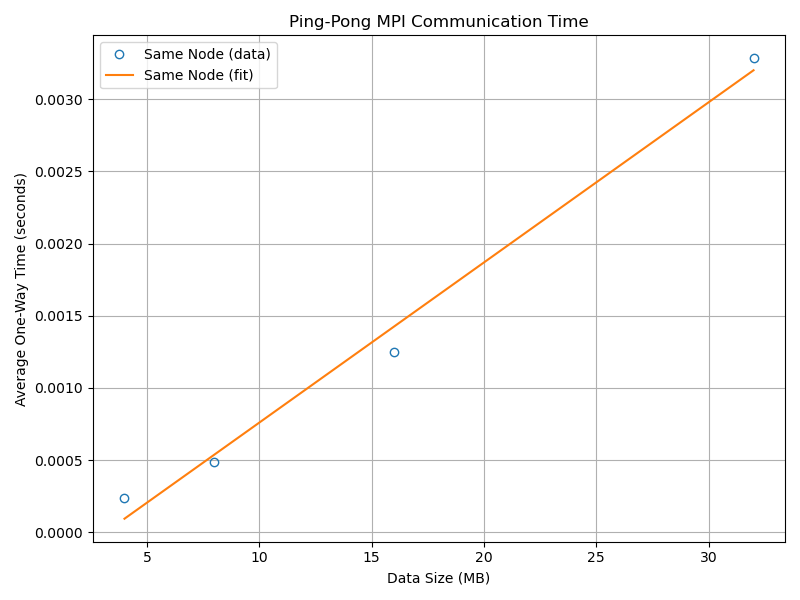
\includegraphics[width=10cm]{./img/pingpong_same_plot.png}
\captionof{figure}{Linear Regression for same}
\end{center}

\begin{center}
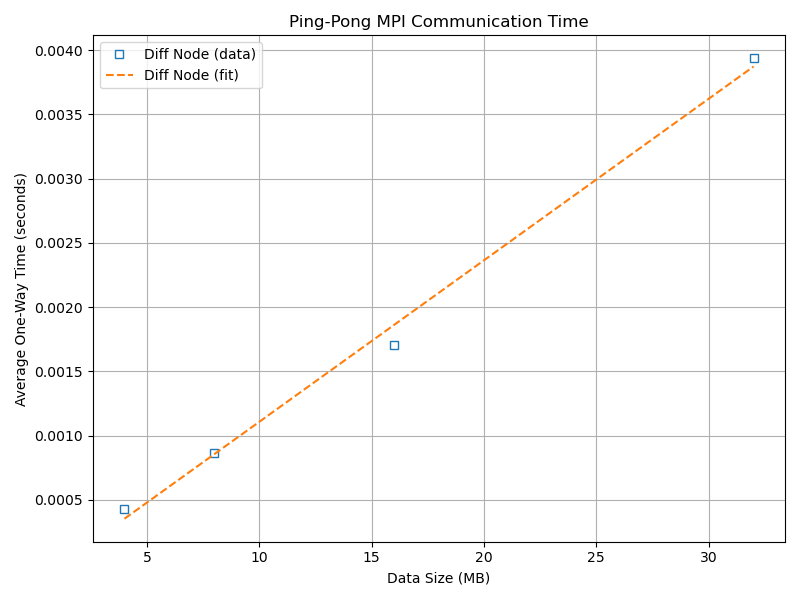
\includegraphics[width=10cm]{./img/pingpong_diff_plot.png}
\captionof{figure}{Linear Regression for diff}
\end{center}

\begin{center}
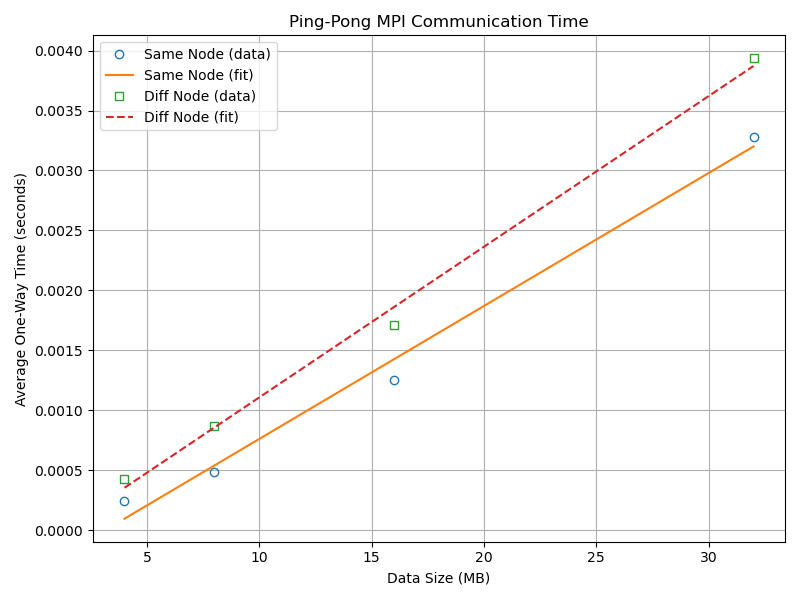
\includegraphics[width=10cm]{./img/pingpong_communication_plot.png}
\captionof{figure}{Linear Regression for both methods}
\end{center}
\newpage
\section{Problem 2}
\label{sec:orgd5b4dd0}
\subsection{Wall-clock Time Table}
\label{sec:orgb07f4fd}

\begin{table}[htbp]
\caption{Problem 2 Wall-clock Time Table}
\centering
\begin{tabular}{|l|c|c|c|}
\hline
Array size & 262144 & 524288 & 1048576\\
\hline
serial & 0.000902495 & 0.001672294 & 0.003332579\\
\hline
2 processes & 0.002470 & 0.005453 & 0.008972\\
\hline
4 processes & 0.003374 & 0.004037 & 0.008923\\
\hline
8 processes & 0.003583 & 0.003975 & 0.008298\\
\hline
\end{tabular}
\end{table}
\subsection{Speedup}
\label{sec:orgd56ea16}

\begin{table}[htbp]
\caption{Problem 2 Speedup Table}
\centering
\begin{tabular}{|l|c|c|c|}
\hline
Array size & 262144 & 524288 & 1048576\\
\hline
2 processes & 0.3652 & 0.3067 & 0.3714\\
\hline
4 processes & 0.2673 & 0.4143 & 0.3733\\
\hline
8 processes & 0.2518 & 0.4205 & 0.4016\\
\hline
\end{tabular}
\end{table}
\subsection{Efficiency}
\label{sec:orgb14973e}

\begin{table}[htbp]
\caption{Problem 2 Efficiency Table}
\centering
\begin{tabular}{|l|c|c|c|}
\hline
Array size & 262144 & 524288 & 1048576\\
\hline
2 processes & 0.1826 & 0.1534 & 0.1857\\
\hline
4 processes & 0.0668 & 0.1036 & 0.0933\\
\hline
8 processes & 0.0315 & 0.0526 & 0.0502\\
\hline
\end{tabular}
\end{table}
\subsection{Discussion}
\label{sec:orgbab6b84}

Speedup is sub-linear due to communication overhead in MPI. Efficiency drops with increasing process count. With 8 processes and 262144 elements, we've got around 3\% efficiency, which suggests that parallel overhead dominates the computation.

The program shows poor scalability especially for small vector sizes. An MPI limitation here is, for lightweight computations, the communication overhead quickly outweighs parallel benefits. Scalability improves slightly with larger input sizes but remains insufficient.
\newpage
\section{Problem 3}
\label{sec:org07b8267}
\subsection{Runtimes}
\label{sec:org5508f65}

\begin{table}[htbp]
\caption{Problem 3 Runtimes}
\centering
\begin{tabular}{|l|c|c|c|}
\hline
Array size & 262144 & 524288 & 1048576\\
\hline
4 processes on the same node & 0.019300 & 0.040307 & 0.084053\\
\hline
4 processes on 4 different nodes & 0.026653 & 0.042971 & 0.112452\\
\hline
\end{tabular}
\end{table}
\subsection{Speedup}
\label{sec:org87b4e3b}

\begin{table}[htbp]
\caption{Problem 3 Speedup}
\centering
\begin{tabular}{|l|c|c|c|}
\hline
Array size & 262144 & 524288 & 1048576\\
\hline
Diff vs Same Speedup & 0.7245 & 0.9370 & 0.7474\\
\hline
\end{tabular}
\end{table}
\subsection{Efficiency}
\label{sec:org449faab}

\begin{table}[htbp]
\caption{Problem 3 Efficiency}
\centering
\begin{tabular}{|l|c|c|c|}
\hline
Array size & 262144 & 524288 & 1048576\\
\hline
Efficiency (Diff Node, /4) & 0.1811 & 0.2343 & 0.1868\\
\hline
\end{tabular}
\end{table}
\subsection{Discussion}
\label{sec:orgaba21be}

MPI Merge Sort shows better scalability on the same node due to reduced communication latency and faster memory access.

Performance drops on different nodes, see in timing and efficiency metrics. This aligns with the other problems results, meaning that distributed-node latency and bandwidth penalty strongly algorithms. Moreover, merge sort algorithm has a significant data exchange.
\newpage
\section{Problem 4}
\label{sec:org1e20f56}

\subsection{Runtimes}
\label{sec:orgdc0bfe8}

\begin{table}[htbp]
\caption{Problem 4 Runtimes}
\centering
\begin{tabular}{|l|c|c|c|c|c|}
\hline
Array size & 1 & 2 & 4 & 8 & 16\\
\hline
Runtime & 0.002640 & 0.001349 & 0.000798 & 0.000388 & 0.000290\\
\hline
\end{tabular}
\end{table}
\subsection{Speedup}
\label{sec:orgee9c0e3}

\begin{table}[htbp]
\caption{Problem 4 Speedup}
\centering
\begin{tabular}{|l|c|c|c|c|c|}
\hline
Processes & 1 & 2 & 4 & 8 & 16\\
\hline
Speedup & 1.0000 & 1.9570 & 3.3075 & 6.8041 & 9.1034\\
\hline
\end{tabular}
\end{table}
\subsection{Efficiency}
\label{sec:orgb72db9b}

\begin{table}[htbp]
\caption{Problem 4 Efficiency}
\centering
\begin{tabular}{|l|c|c|c|c|c|}
\hline
Processes & 1 & 2 & 4 & 8 & 16\\
\hline
Efficiency & 1.000 & 0.978 & 0.827 & 0.850 & 0.569\\
\hline
\end{tabular}
\end{table}
\subsection{Discussion}
\label{sec:org8123224}

The Monte Carlo pi estimation program in strongly scalable. There is small communication overhead, pracitcal speedup around the theorical speedup and a high efficiency.
\end{document}
